%%% Clinic Statement of Work Template
%%%
%%% C.M. Connelly <cmc@math.hmc.edu>
%%%
%%%  $Id: statement-of-work-template.tex 353 2010-08-23 23:47:44Z cmc $


%%% !!! HMC STUDENTS SHOULD REMOVE THE FOLLOWING COPYRIGHT NOTICE FROM
%%% !!! FINAL SUBMISSIONS.

%%% Copyright (C) 2004-2010 Department of Mathematics, Harvey Mudd College.
%%%
%%% This file is part of the hmcclinic class document provided to
%%% HMC mathematics students.
%%%
%%% See the COPYING document, which should accompany this
%%% distribution, for information about distribution and
%%% modification of the document and its components.

%%% !!! END COPYRIGHT NOTICE.


%%% Clinic reports use the clinic class, which should be located
%%% somewhere in TeX's search path.

%%% For your ``statement of work'' (or ``work statement''), specify
%%% the ``proposal'' document-class option to the hmcclinic class.
\documentclass[midyear]{hmcclinic}
\usepackage{graphicx}

%%% The major difference between the statement of work and a midyear
%%% or final report is that the statement of work is typeset as an
%%% article, which means that the highest level of structural
%%% division available to you is section rather than chapter.

%%% There are also some changes in pagination styles and content
%%% that reflect the briefer nature of the proposal.  For example,
%%% in the longer reports, you use \frontmatter, \mainmatter, and
%%% \backmatter to separate some sections of the report from
%%% others.  In the statement of work, you don't need those
%%% commands, as no such division is necessary.

%%% Other packages needed by your document may be loaded here.
% \usepackage{url}              % For formatting URLs and other web or
                                % file references.

%%% Provide additional context around errors. 
\setcounter{errorcontextlines}{1000}


%%% Information about this document.

%%% I find it most useful to put identifying information about a
%%% document near the top of the preamble.  Technically, this
%%% information must precede the \maketitle command, which often
%%% appears immediately after the beginning of the document 
%%% environment.  Placing it near the top of the document makes it
%%% easier to identify the document, and keeps it out from getting
%%% mixed up with the real meat of the document.

%%% We use the same set of commands for specifying information about
%%% the people involved with the project that are used in the longer
%%% reports, so you can copy most of this information directly into
%%% your midyear and final reports.

%%% So, some questions.

%% What is the name of the company or organization sponsoring your project?
\sponsor{SpaceX}

%% What is the title of your report?
\title{Process Time Analysis In Spaceflight}

%% Who are the authors of the report (your team members)?  (Separate
%% names with \and.)
\author{Wendy Brooks~(Fall Project Manager) \and May Lynn Forssen~(Spring Project Manager) \and Alix Joe \and
Rachel Macfarlane}

%% What is your faculty advisor's name?  (Again, separate names with
%% \and, if necessary.)
\advisor{Ben Wiedermann}

%% Liaison's name or names?
\liaison{Jesse Keller \and Jessica Hester \and Jim Gruen}

%%% End of information section.

%%% New commands and environments.

%%% You can define your own commands and environments here.  If you
%%% have a lot of material here, you might want to consider splitting
%%% the commands and environments into a separate ``style'' file that
%%% you load with \usepackage.

\newcommand{\coolcommand}[1]{#1 is cool.} % Lets everyone know that
                                % the person or thing that you provide
                                % as the argument to the command is
                                % cool.


%%% Some theorem-like command definitions.

%%% The \newtheorem command comes from the amsthm package.  That
%%% package is loaded by the class file.

%%% Note that these definitions have changed from the version in the
%%% sample report document by dropping the ``within'' argument.  See
%%% Gratzer's _Math into LaTeX_ or the AMS-LaTeX documentation for
%%% more details.

% \newtheorem{thm}{Theorem}
% \newtheorem{Theo1}{Theorem}
% \newtheorem{Theo2}{Theorem}
% \newtheorem{Lemma}{Lemma}


%%% If you find that some words in your document are being hyphenated
%%% incorrectly, you can specify the correct hyphenation using the
%%% \hyphenation command.  Note that words are separated by
%%% whitespace, as shown below.

\hyphenation{ap-pen-dix wer-ther-i-an}


%%% The start of the document!

%% The document environment is the main environment in any LaTeX
%% document.  It contains other environments, as well as your text.

\usepackage{float}
\restylefloat{table}
\begin{document}

%%% In a longer document (such as your midterm and final reports),
%%% you would have separate \frontmatter, \mainmatter, and
%%% \backmatter commands to define some large chunks of your
%%% document.  For the Statement of Work, which is a short document,
%%% we don't need these commands.

%%% Your Statement of Work begins with a title page.  The title page
%%% is formatted by commands in the document class file, so you
%%% don't need to worry about what it looks like -- just putting the
%%% \maketitle command in your document (and filling in the necessary
%%% information for the identification commands above) is enough.
\maketitle

%%% In a longer document or an article being submitted to a journal
%%% or conference, you would probably have an abstract that
%%% summarized the purpose of the document.  We don't need that for
%%% a Statement of Work.

%%% Similarly, in longer documents you would probably have commands
%%% to include a table of contents and lists of figures or tables.
%%% For a short document such as the Statement of Work, we don't
%%% need these commands.


%%% Content.
\section{Introduction} % May Lynn
SpaceX is an American space transport company that designs and manufactures
advanced rockets and spacecrafts. The eventual goal of the company is to allow
people to live on other planets. SpaceX rockets depend on a variety of software
to be successful, including simulations, flight software, and data analysis.
Almost of this software is written in-house and is complex enough that subtle
problems are often hard to catch and very time consuming to debug.

\section{Background} % May Lynn
\subsection{Tracing and Debugging}
The data that SpaceX developers examine in order to find software bugs is called a kernel trace, which documents the different programs running on a computer over a certain span of time, keeping track of when each program was running on each processor. 

In order to find potential bugs in their software, SpaceX developers look for problems like unexpected preemptions, priority inversions, and breaks in the pattern of programs being run. A preemption occurs when one program is running, and is then blocked by another program starting to run on the same CPU. A priority inversion occurs when a high-priority program is indirectly blocked by something of lower priority using up a shared resource that the higher priority program needs in order to run. The software running on SpaceX rockets has deadlines for programs at regular intervals because timing is very important in rocket flight, so when there is a break in this cyclical pattern of processes this means that there is likely a bug in the software.
\subsection{Existing Tool}
SpaceX currently uses a tool called kernelshark to visualize this trace data and help find any bugs or anomalies. We were informed by our liaisons that this debugging process can take up to several days, so searching for bugs using this tool uses up a lot of valuable time. Much of the user expeience of kernelshark is outdated or could use improvements. The kernelshark tool consists of a graphical display of the programs running on a computer over time, as well as a tabular view of the same information, in the form of CPU events such as processes switching, waking, or sleeping.
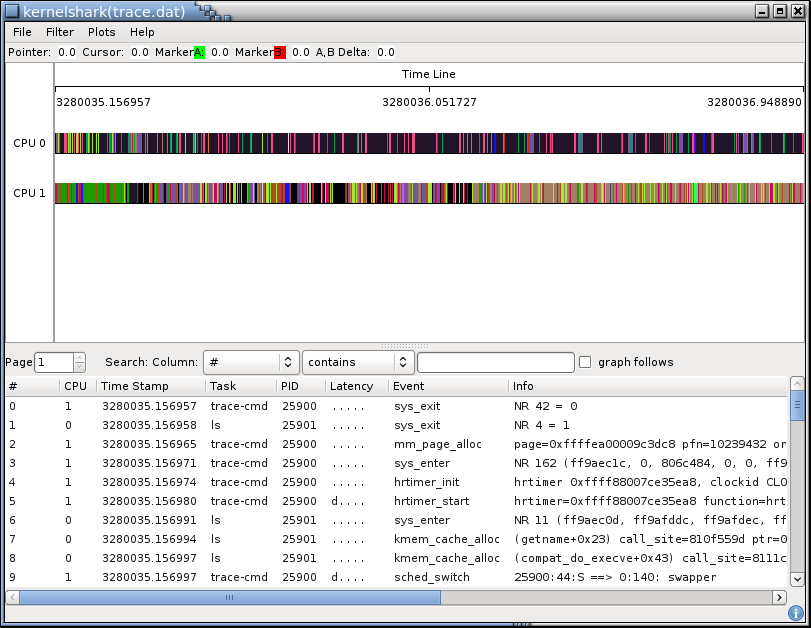
\includegraphics[width=5in]{kshark-open.png}\\
\\
Using only this visualization, it can be difficult to see where the cyclical deadlines for the programs begin and end, making it hard to find when something misses a deadline. In addition, the tabular display of the CPU events in the bottom part of the screen has minimal search functionality and the different columns of the table are not sortable.

\section{Problem Statement} % May Lynn
Our team will make it easier and faster for SpaceX engineers to find software problems by creating a tool that visualizes rocket data and highlights problem areas. We will create an improved user experience and provide more visualizations of the data than the old tool.

\section{SpaceShark}
\subsection{Design}
\subsection{Architecture}
\subsection{Parser}

\section{User Feedback}
\subsection{General Feedback}
\subsection{Feedback on Specific Pages}

\section{Challenges}
\subsection{trace-cmd versioning} % Rachel
  As already described, we collect data using a command-line utility called
  trace-cmd. trace-cmd records various events in the Linux kernel while it runs
  and then outputs this information into a data file with a particular binary
  format. trace-cmd also has a ``report'' option, which takes an existing trace
  file and generates a human readable report of this record. Using this format
  as a starting point instead of the raw binary format simplifies parsing.
  We decided to leverage trace-cmd report instead of wrestling with the binary
  data ourselves. This allowed us to make progress faster and to avoid working
  on an already solved problem.

  Unfortunately, the format of the file generated by trace-cmd report is
  dependent on the version of trace-cmd used. For example, the formatting of the
  ``extra info'' field of a switch event is liable to change. We use this
  field to identify preemptions. To be able to reliably parse data and add
  additional information about preemptions, we need our input data to have
  a consistent format. This creates a dependency on a particular version
  of trace-cmd. Our liaisons have been using trace-cmd version 2.2.1, so
  our parser expects input data to be in the format of 2.2.1.
\subsection{Selection of charting tool} % Rachel
  We chose to use web technologies because we felt there was a wealth of
  charting and UI/UX tools that we could use. We spent several weeks
  experimenting with different charts for the main page. The main page renders a
  timeline of running tasks, which is essentially a large number of colored
  bars. This chart needed to be responsive to zooming and dragging, and to
  dealing with click events to move to a particular time in the table of events
  displayed below it.
\subsection{Batch loading}

\section{Future Work}
\subsection{Known bugs}
\subsection{Extensions}
\subsection{Scalability}
\subsection{more user testing - results}

\end{document}



